\section{Matched forecasting evaluation}\label{sec:experiment}

\subsection{Comparison procedures}


The primary candidate is the bounded KAHM departure. Its five primary
comparators are the common features, bounded RBF departure, raw-history
RBF forecasting, histogram gradient boosting, and a validation-selected
non-KAHM procedure. Raw ridge, persistence, and KAHM and RBF variants that
omit only the departure bound complete the ten-method comparison.
The principal experiment uses the bounded features and fixed geometry
defined in Sections~\ref{sec:reconstruction-method}
and~\ref{sec:bounded-decoder}. All non-ridge candidates are calibrated on C by blending their forecasts
with the same ridge baseline. The selection policy chooses one complete,
calibrated non-KAHM procedure using horizon-averaged normalized C error;
neither KAHM variant is eligible. Raw RBF and boosting have the same
A/B/C roles and horizon-specific hyperparameter selection.
Appendix~\ref{app:reconstruction-results} specifies their grids and costs.

\subsection{Observation laws and independent evaluation roles}

The experiment comprises four laws, two additional-noise levels, and
24 independent repetitions, giving 192 task suites. The nonlinear laws
are an autoregression, Van der Pol dynamics, and Duffing dynamics. A
stable linear Gaussian AR(2) process provides a negative control.
Additional Gaussian observation noise has standard deviation $\eta s_A$,
where $s_A$ is the standard deviation of all original A episode values
and $\eta\in\{0,0.1\}$. The added noise affects histories and targets.
Underlying episodes, standardized noise draws, retained rows, and fitting
seeds are paired between the two noise levels. The oscillator observations
already contain sensor noise when $\eta=0$.

Sets A, B, C, and D contain 64, 32, 32, and 128 episodes, respectively,
each of length 72. Their base episodes and standardized noise draws use
independent random streams; the additional-noise amplitude is estimated
on A and shared across sets. Histories have length 12, horizons are
$\mathcal H=\{1,4,12\}$, and consecutive forecast origins are four
steps apart. A, B, and C retain at most 512, 256, and 256 histories,
respectively; D retains all 1,664 origins. The protocol, executable source,
analysis, and prepared inputs were recorded before reserved forecasts
were computed. This was a prospective local specification informed by
earlier studies, rather than public preregistration or external
replication. Results from other studies are not pooled with this one.


\begin{table}[t]
\centering\small
\caption{Data roles in each principal task suite. Each episode has 72
observations. A history contains 12 observations and predicts horizons
1, 4, and 12. The final evaluation set is not used to choose any model
setting or correction weight.}
\label{tab:data-roles}
\begin{tabular}{@{}lrrp{0.54\linewidth}@{}}
\toprule
Set & Episodes & Histories & Role \\
\midrule
A & 64 & 512 & Fit scalers, reference geometry, baseline, and candidate decoders. \\
B & 32 & 256 & Choose hyperparameters separately for each forecast horizon. \\
C & 32 & 256 & Choose correction weights and one complete non-KAHM procedure. \\
D & 128 & 1,664 & Evaluate fixed forecasts and compute the reported losses. \\
\bottomrule
\end{tabular}
\end{table}

\subsection{Loss aggregation and simultaneous inference}

For task $\tau$, method $m$, and horizon $h$, let
$\MSE_{D,\tau,m,h}$ be the mean squared error over D origins. Define
$v_{\tau h}=\max\{\Var_{A,\tau}(Y_h),10^{-12}\}$, where $Y_h$
denotes the horizon-$h$ target and the
variance uses the retained A target rows with divisor $n_A$. The task loss is
\[
 L_{\tau m}=\frac1{|\mathcal H|}\sum_{h\in\mathcal H}
       \frac{\MSE_{D,\tau,m,h}}{v_{\tau h}}.
\]
For repetition $r$, let $L^{\mathrm{NL}}_{rm}$ average the six nonlinear
law--noise task losses equally, and let $L^{\mathrm{lin}}_{rm}$ average
the two linear-control task losses. For each of the five nonlinear
comparators, define the useful-improvement contrast
\[
 d_{rm}=0.97L^{\mathrm{NL}}_{rm}-L^{\mathrm{NL}}_{rK}.
\]
A positive population mean of this contrast corresponds to an improvement
in expected normalized loss exceeding the specified 3\% margin.
The linear-control contrast is
\[
 d_{r,\mathrm{lin}}=1.05L^{\mathrm{lin}}_{r,\mathrm{ridge}}
                          -L^{\mathrm{lin}}_{rK},
\]
which tests noninferiority with a 5\% relative tolerance. For each
contrast, $\bar d=24^{-1}\sum_r d_r$ and
$s_d^2=23^{-1}\sum_r(d_r-\bar d)^2$ denote the sample mean and variance.
The one-sided lower confidence bound is
\[
 \bar d-t_{23,1-0.05/6}\,\frac{s_d}{\sqrt{24}},
\]
where $t_{\nu,q}$ is quantile $q$ of the Student $t$ distribution with
$\nu$ degrees of freedom. Bonferroni adjustment covers the six contrasts
simultaneously at nominal level 95\%, subject to the paired-mean
$t$ approximation. The sampling units are independent repetition
aggregates; overlapping windows and paired noise levels do not increase
the inferential sample size.

The prespecified criterion requires all six lower bounds to exceed zero.
It also requires complete finite predictions, satisfaction of the
feature, coefficient, and correction bounds, and a taskwise maximum
absolute KAHM error no greater than five times the corresponding ridge
maximum. The last requirement is an engineering diagnostic rather than
a population risk guarantee. A wholly failed method or a final
prediction-cell recovery prevents an efficacy conclusion. The 3\%
improvement margin, 5\% tolerance, and fixed 24-repetition budget express
the study's research criteria; they do not derive from a deployment loss
function or a power calculation. Failure to satisfy the complete criterion
concludes the planned performance evaluation without adding repetitions
or selecting favorable conditions after inspecting D.

\subsection{Predictive results}

The bounded KAHM departure has nonlinear aggregate NMSE $\RMKNonlinearNMSE{}$.
Its point relative gains over the common basis, matched bounded RBF departure, raw RBF, boosted trees and C-selected policy are
$\RMKvsCommonGain{}\%$, $\RMKvsRBFDepartureGain{}\%$, $\RMKvsRawRBFGain{}\%$, $\RMKvsBoostingGain{}\%$ and $\RMKvsPolicyGain{}\%$, respectively.
Positive values denote smaller mean KAHM loss; these percentages are point estimates, not confidence bounds.
1 of the five useful-superiority conditions pass, and the linear-control noninferiority condition passes.
Every declared feature, coefficient, correction and maximum-error screen passes.
The comparison with the common basis establishes useful aggregate value for this bounded reconstruction-and-decoder procedure under the declared margin.
The frozen decision is therefore to \emph{stop this forecasting-performance branch}.
The complete required KAHM-specific predictive advantage is not established at the chosen budget. This does not prove equivalence, make all reconstruction features useless, or establish impossibility for every time-series law.
A favorable descriptive law, noise level or horizon cannot replace the aggregate specified before evaluation.


\begin{table}[t]
\centering\small
\setlength{\tabcolsep}{3.5pt}
\caption{The six primary comparisons for bounded KAHM departure.
$L_K$ and $L_m$ are losses averaged over repetitions. The first five rows
use the nonlinear aggregate and $\bar d=0.97L_m-L_K$; the last uses
the linear aggregate and $\bar d=1.05L_m-L_K$. Gain is
$100(1-L_K/L_m)$, so negative values favor the comparator. The lower
bound concerns the absolute margin contrast, not the percentage gain.
All bounds use 24 independent repetitions, 23 degrees of freedom, and
a one-sided Bonferroni adjustment for six comparisons. A criterion is
satisfied only when its lower bound is positive.}
\label{tab:mechanism-primary}
% Generated from the complete saved reconstruction-mechanism analysis.
\begin{tabular}{@{}lrrrrrc@{}}
\toprule
Comparator & $L_K$ & $L_m$ & Gain (\%) & $\bar d$ & Lower bound & Pass \\
\midrule
Common basis & 0.02993 & 0.03423 & 12.58 & 0.00328 & 0.00295 & Yes \\
RBF departure (bounded) & 0.02993 & 0.03028 & 1.17 & -0.00055 & -0.00079 & No \\
Raw RBF & 0.02993 & 0.03115 & 3.92 & 0.00029 & \ensuremath{-8.286\times10^{-5}} & No \\
Boosted trees & 0.02993 & 0.02941 & -1.77 & -0.00140 & -0.00194 & No \\
C-selected non-KAHM policy & 0.02993 & 0.02822 & -6.04 & -0.00255 & -0.00299 & No \\
Linear control: ridge & 0.89810 & 0.89632 & -0.20 & 0.04303 & 0.04161 & Yes \\
\bottomrule
\end{tabular}

\end{table}

The improvement over the common basis shows that the bounded
reconstruction departure provides useful functions to this decoder.
The matched RBF reconstruction provides much of the same benefit:
KAHM's point improvement over it is below the 3\% margin. KAHM's
point improvement over raw RBF exceeds 3\%, but the simultaneous lower
bound remains below zero, leaving that margin unresolved. Boosting and
the selected non-KAHM procedure have smaller aggregate point losses.
Thus the results support reconstruction features without establishing
the required practical advantage specific to KAHM.

Figure~\ref{fig:mechanism-conditions} shows every law and noise level
for the matched reconstruction control and the selected non-KAHM
procedure. These descriptive comparisons show how the relative error
varies across the declared conditions. The appendix gives all ten
methods, and the accompanying data include every horizon-specific result.

\begin{figure}[t]
\centering
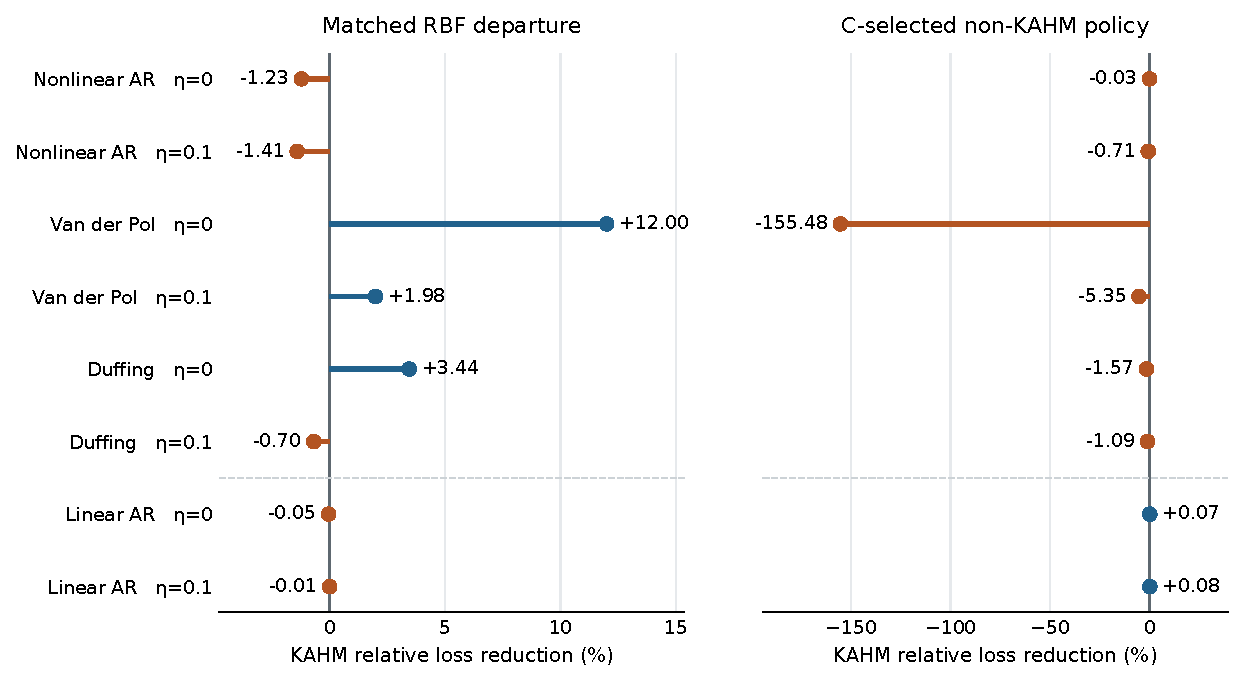
\includegraphics[width=\linewidth]{generated/reconstruction_mechanism/law_noise_contrasts.pdf}
\caption{Condition-specific gains of bounded KAHM departure over the
matched bounded RBF departure and the C-selected non-KAHM procedure.
Each point is $100(1-\overline L_K/\overline L_m)$, where the bars denote
mean loss over 24 repetitions of that condition. Positive values favor
KAHM. The panels use different horizontal scales, and labels give the
point estimates. These descriptive estimates have no condition-specific
confidence claims. The dashed divider separates nonlinear laws from
the linear negative control.}
\label{fig:mechanism-conditions}
\end{figure}

\subsection{Numerical checks and measured resources}

The maximum taskwise KAHM-to-ridge maximum-error ratio is
\RMMaxErrorRatio{}, below the limit of five. There are
\RMFeatureViolations{} feature-bound, \RMCoefficientViolations{}
coefficient-bound, and \RMCorrectionViolations{} correction-bound
violations. C selects a nonzero KAHM correction weight in
\RMKActiveNonlinear{} of 432 nonlinear task--horizon combinations and
\RMKActiveLinear{} of 144 linear-control combinations. This activation
frequency describes calibration choices, not a guarantee of lower D loss.
Mean charged fitting and selection time is \RMKFitSeconds{} seconds
for bounded KAHM departure and \RMRFitSeconds{} seconds for bounded RBF
departure. Appendix~\ref{app:reconstruction-results} reports prediction
time, retained model size, and the accounting boundaries.

The algebraic example, deterministic bound, and empirical comparisons
answer different questions. A distinct feature can be poorly aligned
with the target or difficult to estimate from the available sample.
A bounded correction can remain inaccurate. An unresolved improvement
margin does not establish equality of the representations. The
conclusions therefore apply to the specified reconstructions, decoder,
selection rules, and observation laws.
